\chapter{Documents d’analyse}

\begin{figure}[h]
  \centering
  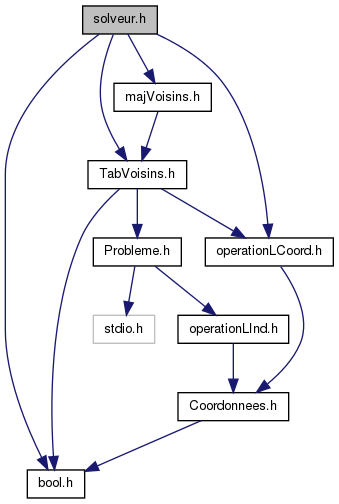
\includegraphics[scale=0.5]{solveur-dependance}
  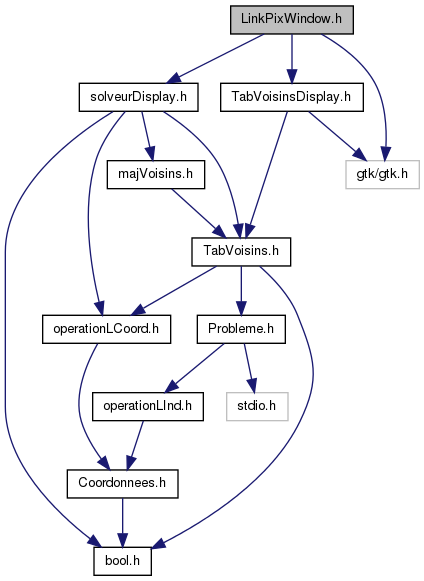
\includegraphics[scale=0.5]{link-pix-window-dependance}
  \caption{Graphe des dépendances du solveur à gauche et de du solveur graphique à droite}
  \label{graphes-dependance}
\end{figure}

Les fichiers \verb$solveur.h$ et \verb$solveur.c$ ne sont pas utilisés dans le cadre du logiciel, mais sont conservés car ils contiennent le solveur en un seul morceau (et non pas des itérations découpées comme dans \verb$solveurDisplay.h$ et \verb$solveurDisplay.c$, qui sont des adaptations du solveur pour la surcouche graphique).
